\chapter{具备交易金额隐私保护的支付方案设计}

本章节从模型中的安全需求出发,分析交易金额隐私保护的需求,并依据需求设计交易方案,对交易方案的安全假设、交易过程等进行文字上的描述。

\section{设计目标}

本文提出的对交易金额进行隐私保护的交易方案,其核心安全设计目标为“在确保交易正常进行的情况下,使得交易信息中的交易金额不被不可信第三方知晓”,此外还有一些次级的目标和需求。这些需求可以细分拓展为下面几个部分:

\begin{enumerate} % ... 和后文对应!
    \item 交易金额的隐私性。该需求为核心设计目标。单笔转账必然经过某一支付服务提供商,而该服务商必须在不知晓具体金额的前提下,完成对交易的处理。
    \item 交易的正确性。对于单笔转账,需要确保转出方公钥加密的密文,和转入方公钥加密的密文,其对应的明文是一致的。此外,还需要通过某种途径,确保交易的金额不会超过转出方的余额。
    \item 交易的不可伪造性。对于单笔交易,转出者需要确保该交易是由其授权的,而不是由恶意第三方伪造的。换句话说,支付服务提供商能够确认该交易是确实由转出方授权的。
    \item 建立客户端与服务端之间的网络通信。交易信息需要通过网络传输,且本文方案中客户端与服务端的交互需要经过互联网,因此需要设计网络通信的方式。
    \item 对交易信息的访问。鉴于在本方案中,只需要保护交易金额,而不需要保护交易的其他信息,且本方案将允许在不进行鉴权的情况下,获取交易信息的密文数据。因此,选择一种具有较高的安全性的加密方案,且能够对抗可能的量子计算的威胁是必要的。
    \item 服务方对手续费的收取。在现实中,支付服务提供商通常会对交易进行一定的交易手续费的收取,以保证服务的持续性。因此,本方案需要为服务商能够对密文金额进行手续费计算提供空间。
    \item 交易信息的持久化储存。方案需要允许任意人员对任意交易信息(密文)进行访问,因此需要一种方法,使得服务端作为记账方,能够对交易信息进行存储,尤其是对密文交易金额的存储。
\end{enumerate}

\section{方案构造}

本节将对方案的构造进行说明。基于上述需求,本文提出了一个简单的对交易金额进行隐私保护的交易方案,其构造如下图所示。方案由客户端,包括转出方和转入方,服务端和监管方组成,客户端负责交易的发起,服务端负责交易的接受和验证。客户端和服务端之间通过 HTTP 协议进行通信。监管方作为可信第三方存在,以黑盒的方式,向单笔交易提供验证,同时有能力了解到交易信息。

\subsection{支付场景抽象}

\begin{figure}
    \centering
    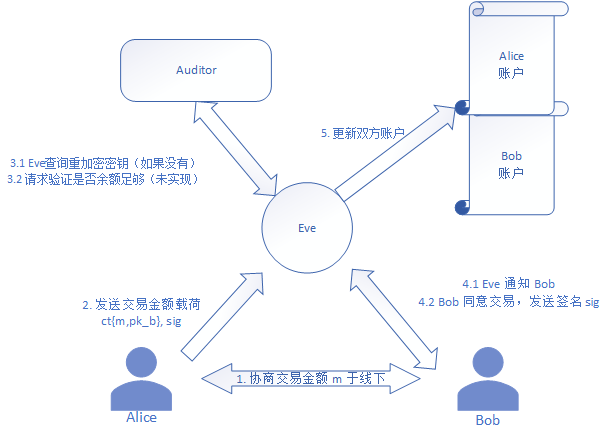
\includegraphics[width=0.8\linewidth]{Figures/chimata-transaction-abstract.png}
    \caption{方案抽象描述}\label{Fig:chimata_abstract_transaction}
\end{figure}

假设付款人 Alice 想要给收款人 Bob 进行一笔金额为 $m$ 的转账,转账操作需要经过支付服务提供方 Eve Corp. 提供的服务。Alice 和 Bob 的公钥分别为 $pk_A$ 和 $pk_B$,私钥分别为 $sk_A$ 和 $sk_B$。

\subsection{基本假设}

\textit{假设 1:} 监管方是绝对安全的,不会向外界透露任何保密信息。该假设使得本方案不考虑监管方受到攻击的可能性,且用户可以无条件信任监管方,将自己的私钥托管给监管方保管,而不需要担心敏感信息泄露。

\textit{假设 2:} 交易双方的交易金额已经在线下商定完毕。该假设意味着本方案无需考虑交易双方具体的,对交易金额的协商过程的保密性,而只需考虑处理交易过程中交易金额的保密性。换句话说,即交易金额不会因本方案以外的因素泄露。

\textit{假设 3:} 服务端具有无限的存储空间。不同于传统公钥密码学的加密方案,为了保证加密的安全性,CKKS 方案的公钥、私钥和密文本身的规模都相对较大\footnote{相对于前人学者的方案已经有了极大的优化,然而由 Lattigo 导出的密钥规模仍然较大,约有数百 KB,无法忽略}。另一方面,密文规模本身会因为维度的增长而增长,意味着密文之间的同态乘法运算会导致密文规模的膨胀。\footnote{本文所提出的方案并不包含密文之间的同态乘法,但是随着方案的拓展仍然为可能的需求留有计算的能力}

\section{完整交易流程}

\subsection*{初始化阶段}

系统输入安全参数 $\lambda$,输出系统的公共安全参数。在本方案中,选择 secp224r1 作为椭圆曲线数字签名算法所使用的曲线,选择 PN12QP109 \footnote{即 $\log N = 12$ 且 $\log QP = 109$,允许对高达 $2^{11}$ 个元素的复向量进行加密} 作为 CKKS 方案所使用的安全参数。Alice 和 Bob 分别使用上述的公共安全参数,生成公私钥链\eqref{eq:Pub_and_Priv}并提交给监管方。

\begin{equation} \label{eq:Pub_and_Priv}
\begin{aligned}
    pk_{Alice}, pk_{Bob} = \{pk_{ECDSA}, pk_{CKKS}\}\\
    sk_{Alice}, sk_{Bob} = \{sk_{ECDSA}, sk_{CKKS}\}
\end{aligned}
\end{equation}

当 Eve 进行查询时,监管方可以通过下列方法\eqref{eq:GenSwkPair}生成重加密密钥,返回给 Eve。

\begin{equation} \label{eq:GenSwkPair}
    GenSwkPair(sk_{Alice}, sk_{Bob}) \rightarrow swk_{Alice \rightarrow Bob},
    swk_{Bob \rightarrow Alice}
\end{equation}

\subsection*{交易的发起和签名阶段}

在该阶段,付款人 Alice 和收款人 Bob 已经在线下商定好交易金额 $m$,将要进行付款。此时 Alice 选择使用 Bob 的公钥对金额进行加密,并对密文进行签名,产出以下密文载荷\eqref{eq:payload}:

\begin{equation} \label{eq:payload}
payload_{Bob} = [ct_{bob}\{m\}, sig_{sk_{Alice}}\{ct_{bob}\{m\}\}]    
\end{equation}

Alice 将自己和 Bob 的唯一识别符,与上述载荷结合,生成一个新的交易载荷并发送给 Eve,等待 Eve 回应,并由 Eve 进行后续操作。

需要注意的是,Alice 也可以使用自己的公钥进行加密,并产生载荷,此时该交易不需要 Bob 进行确认而直接记账,过程与下文相似,本文不再赘述。

\subsection{交易的验证和处理}

Eve 此时接收到 Alice 的转账请求,其首先验证 Alice 转账的真实性。Eve 对载荷中的 $sig_{sk_{Alice}}\{ct_{bob}\{m\}\}$ 使用 Alice 的公钥进行验证,即执行方法\eqref{eq:Verify_1}。

\begin{equation} \label{eq:Verify_1}
    Verify(ct_{bob}\{m\}, pk_{Alice}, sig_{sk_{Alice}}\{ct_{bob}\{m\}\})
\end{equation}

若验证为真,则说明该交易是 Alice 发起的,且 Alice 确实想要将 $ct_{bob}\{m\}$  对应的明文金额转给 Bob。若验证为假,则说明该交易并非由 Alice 发起,Eve 应当拒绝该交易,返回状态码 401\footnote{Unauthorized,用于标记鉴权失败} 并停止处理。

在验证真实性后,Eve 开始处理该笔交易。在向交易输入唯一识别符和状态等元数据后,Eve 使用从监管方处获取到的重加密密钥 $swk_{B \rightarrow A}$ 使用 $SwitchKey_{swk}$ 函数将 Alice 提交的密文 $ct_{bob}\{m\}$ 转换为 $ct_{alice}\{m\}$,并进行手续费的计算。随后 Eve 将交易写入数据库,向 Alice 反馈状态码 200,并返回该交易目前的信息。Eve 同时向 Bob 发送一条消息,等待 Bob 的确认。

\subsection*{交易的接受}

在该阶段,Bob 接收到了来自 Eve 的通知,需要对该交易进行接受。

首先,Bob 可以选择对该交易进行独立的验证,包括对金额密文 $ct_{bob}\{m\}$ 进行解密验证,以及对 Alice 的签名进行验证。Bob 可以选择接收该交易,也可以选择拒绝\footnote{即忽略该交易,等待交易自动过期}。

若 Bob 选择接收交易,则此时 Bob 需要对 Alice 的密文进行签名,产生以下载荷\eqref{eq:Payload_bob}:

\begin{equation} \label{eq:Payload_bob}
    payload_{Alice} = [ct_{Alice}\{m\}, sig_{sk_{Bob}}\{ct_{Alice}\{m\}\}]
\end{equation}

Bob 将上述载荷连同该笔转账的唯一标识符发送给 Eve,等待 Eve 返回记账成功的应答。该操作标志着 Bob 亦认可该项交易。

\subsection{交易的最终记账}

Eve 在收到 Bob 的确认后,从数据库提取该未完成交易的信息,并进行处理。该阶段 Eve 首先对签名进行验证,执行函数\eqref{eq:Verify_2}。若验证为真,则开始更新双方余额,并写入数据库;若验证失败,则停止处理并返回 401 

\begin{equation} \label{eq:Verify_2}
    Verify(ct_{Alice}\{m\}, pk_{Bob}, sig_{sk_{Bob}}\{ct_{Alice}\{m\}\})
\end{equation}

当 Eve 完成所有处理后,向 Bob 返回状态码 200,并附带该笔交易的所有信息。此时,Alice 和 Bob 都可以以交易的标识符向 Eve 查询该交易信息。

\section{方案分析}

\subsection{交易隐私性分析}

本方案的重点在保护交易金额不被第三方支付平台了解到,因此,本方案使用 CKKS 方案对用户交易信息中的交易金额进行加密,而这些密文如果没有私钥则无法解密。

% (NOT A) TODO (Anymore): 需要更详细,更形式化的说明
具体而言,CKKS 方案所基于的困难问题,即 R-LWE 问题,在其被提出的文献\cite{cryptoeprint:2012/230}中被证明是和 SVP 等价的,而后者已经被证明是 NP 困难的问题\cite{10.1145/276698.276705}。对于攻击者而言,其无法在没有私钥 $sk$ 的情况下对密文 $ct = [ct_0(X), ct_1(X)]$ 进行还原。因此,用户交易金额密文对任何第三方都是无法辨认的,保护了用户交易金额的隐私。

\subsection{交易的正确性分析}

交易的正确性,指的是保证交易双方的密文交易金额所对应的明文是一致的\footnote{然而 CKKS 的特性无法保证完全一致,因此本处指的是在误差范围内一致}。可交易性则指的是支付服务提供方,在不了解交易双方的交易内容和账户明文余额的情况下,仍然能够做到更新双方账户余额,进行手续费计算的操作。

为了确保交易正确性,本文通过文献\cite{brakerski2014leveled}和 Lattigo 提供的密钥交换方法,以重加密的方式确保了两个密文对应明文的一致,其中交换密钥由交易双方私钥组合生成。例如,当我们拥有使用 Alice 的公钥加密的密文 $CT_{A}\{M\}$ 和交换密钥 $swk_{Alice \rightarrow Bob}$,我们就可以执行方法\eqref{eq:SwitchKey},将用 Alice 公钥加密的密文转化为用 Bob 的公钥加密的密文 $CT_{B}\{M\}$。将 $CT_{B}\{M\}$ 进行 解密得到的 $M' = f(M)$ 和原文是处于一定误差内的,在 CKKS 方案中即可以被认为是一致的。

\begin{equation} \label{eq:SwitchKey}
    SwitchKey_{swk_{Alice \rightarrow Bob}}(CT_{A}\{M\}) = CT_{B}\{M\}
\end{equation}

前文\ref{sec:CKKS_Review}提到,CKKS 方案允许对全体浮点数的消息空间进行加密解密和相关同态操作。相关同态性质可被用于确保交易处理过程中的正确性。具体而言,CKKS 的同态加法和乘法可以被用于更新余额:对于余额增加只需要执行一次同态加法,而对于余额减少,需要对交易金额乘以 $-1$ 后进行同态加法。

\begin{equation}
\begin{aligned}
    Sender Balance:  CT_{balance}' & = CT_{balance} - CT_{transaction}\\
    &= CT_{balance} + MultByConst(CT_{transaction}, -1)\\
    Receipt Balance: CT_{balance}' & = CT_{balance} + CT_{transaction}
\end{aligned}
\end{equation}

\subsection{交易真实性分析}

交易的真实性,也被称为不可伪造性,指的是对于单笔交易,转出方能够确保该转出请求是由其授权的,对转入方同理。在本文的方案中,攻击者在不持有私钥 $sk_{ECDSA}$,且依赖的库 \verb|crypto/ecdsa| 被正确地实现的情况下,伪造一个交易签名是困难的。

若攻击者在伪造签名时,需要知道签名者的私钥 $dA$ 和选区的随机数 $k$。从私钥的保密性来看,由前文\ref{sec:ecdsa}可知,由于单向陷门函数的存在,无法从公钥 $Qa$ 反向计算出私钥 $dA$。如果攻击者不知道这些信息,他就无法计算正确的签名。从攻击者仅从公开信息以伪造签名的角度看,若需要伪造签名,则需要解决椭圆曲线离散对数问题\cite{Hankerson2011}和模逆元问题。这两个问题都是困难的。因此,可以认为攻击者无法对交易进行伪造,也就确保了交易的真实性。
